\section{Introduction}
\begin{figure}[htbp]
	\centering
	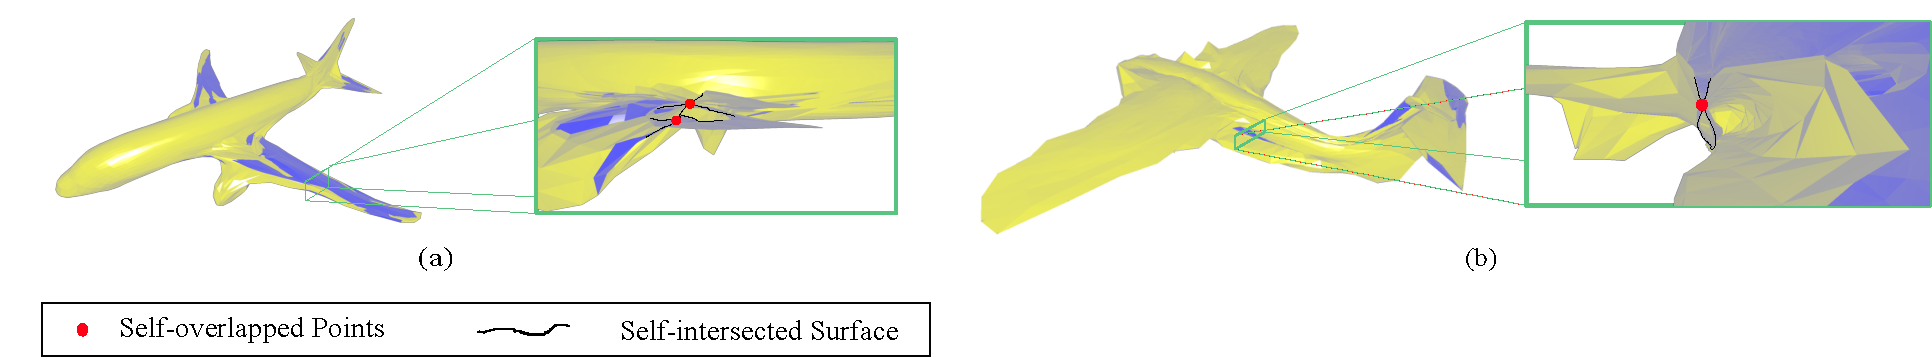
\includegraphics[width=\linewidth]{img/issue/issue}
	\caption{Self-intersections in 3D surface mesh reconstruction networks. (a) A surface mesh of a plane generated by AtlasNet \cite{atlasnet} (sphere as its parameter domain). (b) A surface mesh of a plane generated by Pixel2Mesh \cite{pixel2mesh}. Outside faces are rendered as golden and inside faces are rendered as bluish. \mdf{Some} inside triangles are exposed due to self-intersections. We highlight some self-intersected faces and their corresponding overlapped points in the close-up view.}
	\label{fig:issue}
\end{figure}
%introduction to 3D shape reconstruction from single view
Inferring 3D shape from a single view image is a traditional problem for computer vision. In computer graphics, 3D modeling with a given image has also been extensively studied. In recent years, deep neural networks (\cite{3DR2N2,PSGN,3Drender,imgrecon15,3dshapenet,endface,octreegen,surfnet,shapeprior}) have achieved great success in this field. Unlike classic shape from X (e.g. \cite{shapefromshading,shapefromtext1,shapefromtext2}) approaches, these neural networks are able to recover not only the visible frontal shape but also the invisible part for an object from a single-view color image by learning and representing complicated prior knowledge from a large dataset. 

Existing networks all rely on variants of 2D convolution neural networks to extract information and encode 2D images, but use quite different techniques to represent and decode 3D shapes. Started from 3D ShapeNets \cite{3dshapenet} and greatly improved by introducing octree structure (\cite{octreegen}), volumetric representation and 3D convolutional networks are most commonly used in this problem. There is also a point set generation network (\cite{PSGN}) that uses unordered point set representation and directly regresses a point set using both convolutional and fully connected branches. \cite{endface} employ a bilinear model to represent 3D faces and regress the interpolation coefficients to generate a face shape from an image. \cite{surfnet} explicitly use spherical parameterization as a post-processing stage to represent a 3D shape as a geometry image in the parameter domain. 

%introduction to 3d mesh reconstruction networks-- AtlasNet and Pixel2Mesh to be specific
In latest works, AtlasNet (\cite{atlasnet}) and Pixel2Mesh (\cite{pixel2mesh}) to be specific, a new idea has been applied on this problem. Neural networks are designed to learn the mapping from a predefined surface (square and sphere for AtlasNet and ellipsoid for Pixel2Mesh) to a target surface instead of directly regressing the absolute positions of surface points as in \cite{PSGN}. These methods have shown great potential in generating meshes for generic objects. It is convenient to integrate mesh-related operations and energy functions in these networks. For example, Pixel2Mesh integrates graph-based unpooling and Laplacian regularization in the neural network.

Despite all of these progresses, there are still a lot of issues which prevent network-generated meshes from being useful in many real-world applications. However, we believe deep learning is the most promising approach to integrate more intelligent method in 3D modeling.

%introduction to the self-intersection issue
 In this paper, we address a specific issue that appears in both AtlasNet \cite{atlasnet} and Pixel2Mesh \cite{pixel2mesh}. As shown in Figure~\ref{fig:issue}, the AtlasNet and Pixel2Mesh frequently generate meshes with self-intersected surfaces. This issue appears partially because AtlasNet and Pixel2Mesh employed the Chamfer distance loss, which is used firstly to train the point set generation network (PSGN, \cite{PSGN}). The Chamfer distance loss was designed to measure the discrepancy between two unordered point sets and it does not take surface into consideration. AtlasNet uses Poission surface reconstruction as post-processing or double-sided lighting in rendering to cover up this issue. Pixel2Mesh adopts a coarse-to-fine framework and uses additional losses (i.e. edge length loss, Laplacian loss) in order to alleviate this issue. They all failed to address the essential reason behind this issue, while most efforts in these mesh generation networks have been put on increasing shape details for the generated mesh.

In this paper, we tackle the issue of self-intersection from the essential reason behind it, which is non-injectivity of the predicted mapping. In other words, without injectivity, two points on the predefined surface could be possibly mapped to the same point by the neural network, which leads self-intersection or self-overlapping in the generated surface.
%challenge
To enforce \mdf{local} injectivity, many techniques have been proposed by constraining the Jacobian of the mapping function. \cite{tvcgprevent} have used it to prevent self-intersection in Free-Form Deformation (FFD) of solid or surface meshes. Starting from a mesh that is free from self-intersection, \cite{tvcgprevent} divide FFD into injective sub-steps to avoid self-intersection in the output mesh.

\mdf{Local injectivity} has also been studied in parameterization optimization to prevent folding. For surface with disk topology, one possible strategy is to start from a feasible solution (by Tutte's embedding \cite{tutte} or its variants) and keep every optimization iteration or deformation inside feasible regions. This can be enforced by adding barrier energy from distortion metrics (e.g. \cite{provableplanarmapping,lifted_bijection}), bounding the triangle distortion (e.g.\cite{freeboundary,boundeddistortion})
or using a progressive strategy \cite{Liu_PP_2018}.

It is non-trivial to adopt their strategies for training neural networks, since existing networks learn to predict the mapping for many different shapes simultaneously and only a batch of these shapes are sampled from the dataset in each training iteration. One challenge is to initialize the network parameters to ensure that initial outputs are free of self-intersection for all possible inputs. Another challenge is to alter batch-based optimizer to constrain the deformation of outputs within an injective region for all possible inputs. 

In order to learn injective mapping for meshes, we propose a cycle regularization technique. \mdf{Our technique is deduced from basic decision theorem of injectivity. Therefore it reduces not only local self-intersections but also global self-interferences of the surface.} It is easy to implement by reusing the existing differentiable layers within existing surface mesh reconstruction networks, such as AtlasNet \cite{atlasnet} and Pixel2Mesh \cite{pixel2mesh}.

%our solution
 Our strategy is to use an inverse 3D decoder to learn an inverse mapping from  the target surface back to the source surface along with the forward mapping in the original network. Therefore, a point from the source surface can be mapped to the target surface and then mapped back. We use the difference after such cycle mapping to form our regularization term and we call it cycle regularization. While the network learning a mapping to approximate the target surface, our regularization term \mdf{tries} to ensure that an inverse mapping exists (i.e making the forward mapping injective, as we explain in Sec~\ref{subsec:cyclereg}).
Note that the inverse 3D decoder is only needed in training phase. Therefore, it is a regularization technique which does not increase the complexity of the original neural network for mesh generation.

In summary, our contributions in this paper are three-fold.
\begin{itemize}
	\item We propose a novel cycle regularization technique to prevent self-intersection for surface mesh reconstruction networks. 
	\item We apply our cycle regularization technique on two latest mesh generation networks, AtlasNet \cite{atlasnet} and Pixel2Mesh \cite{pixel2mesh}, showing that our technique keeps the network end-to-end trainable by using existing differentiable layers.
	\item We validate with experiments that when trained with cycle regularization, these networks are able to produce surface meshes with significantly less self-intersection, and still lead to comparable  Chamfer distance between the generated mesh and the ground-truth mesh compared with original networks. 
\end{itemize}

 